\chapter{Modelling Experiments with SCPs} \label{chp:model}
\section{Overview}
As with any cognitive framework, the most important metric for judging the success of SCPs comes from testing how well SCPs can approximate empirical data across tasks. This chapter will show the suitability of SCPs with a common set of allowable cognitive operations for modelling several well-studied experiments in cognitive modelling.

In particular, we will show that the Wason Selection Task, and Suppression Task can be modelled at both the general and individual reasoner level with SCPs in a formulation that is both intuitive and consistent with the WCS approach already described in Chapter~\ref{chp:experiments}. For the Suppression Task we also show that an SCP interpretation using Reiter's Default Logic remains unable to show Suppression in the default theory from Section~\ref{ssec:supReit}.

\section{Suppression Task} \label{sec:supSCP}

\subsection{Suppression Task: WCS}
Whilst modelling the Suprression Task in this section, we will continue to use the notation and variables defined in Section~\ref{sec:sup}. Below is a brief restatement of the phrasing of the problem:

\begin{enumerate}
\item If she has an essay to write ($e$), she will study late in the library ($l$).
\item If the library is open ($o$), she will study late in the library ($l$).
\item She has an essay to write ($e$).
\end{enumerate}

To model the Suppression Task in the SCP framework, we must first define the SCP Task $\Pi_{sup}=(s_i,M,f_\text{sup}(),\gamma)$ which outlines the restrictions and goals of the model. The structure of $s_i$ must be robust enough to capture information regarding a set of rules, variable assignments in the possible world, and conditionals. To this end we define:

\[s_i=\{s_i^\text{el},s_i^\text{elo}\}\]
\[s_i^\text{el}=\{S,\Delta_\text{noSup}, V, \text{name}=\text{`el'}\} \]
\[s_i^\text{elo}=\{S,\Delta_\text{Sup}, V, \text{name}=\text{`elo'}\} \]




For the the only unconditional rule, that she has an essay to write, we define $S=\{(e \leftarrow \top)\}$. The set of conditional rules $\Delta_{\text{noSup}}=\{l|e\}$ captures the probable assumption that she will study late in the library if she has an essay to write, $\Delta_{\text{sup}}=\{(l|e),(l|o)\}$ captures the addition of the conditional that if the library is open she will study late in the library. And the possible world $V=\{(e,u),(l,u),(o,u)\}$ sets all variable names occurring in $S$ and $\delta$ to unknown. The structural variable \textit{name} discriminates the two epistemic states and, because there is no cognitive operation in $M$ which can add, remove or change or change \textit{name}, it is guaranteed that every base point in the final state will have the name `el' or `elo' indicating from which initial epistemic base point it was generated.

The second consideration $M$, denotes the set of possible cognitive operations which may occur in the resulting SCPs and realised SCPs of $\Pi_{sup}$. Following the intuition we used in Section~\ref{sec:sup}, we choose cognitive operations that enable application of the WCS and interpretation of conditionals. To that end we define:

\[
M=\{\texttt{addAB}, \texttt{semantic}, \texttt{wc}\}
\]

The external evaluation function should translate the SCP into a decision that can be compared with empirical data. In the Suppression Task we will treat $f_\text{sup}()$ as a function that makes a single choice from the set $\{$\textit{`she will study late in the library'},\textit{she will not study late in the library}, \textit{we are uncertain if she will study late in the library}$\}$. Under the assumption only the final state point $p_n$ determines whether she will study late, we might define the final state dependant external evaluation function $f_\text{sup}()$ as follows:

\begin{algorithm}[H] 
\SetAlgoLined
\SetKwProg{Fn}{Function}{ is}{end}
\Fn{$\texttt{f}_\text{sup}(\pi)$}
{
\tcc{This is a final state evaluation SCP.}
Let $R=\{(k\in K[\pi],f_\text{sup}())\}$ be the set of realised SCPs of the form $r_i=(k,f_\text{sup}())$ which can be generated from $\pi$.\;
Let $P=\{\bar{p}_1,...,\bar{p}_n\}$, where $\bar{p}_i$ is the final state of $r_i$\;

\tcc{Get all final epistemic state which can be generated from each of the two initial epistemic states}
$P_\text{el}:=\{\bar{p} \in P | \bar{p}[\text{`name'}]=\text{`el'}\}$\;
$P_\text{elo}:=\{\bar{p} \in P | \bar{p}[\text{`name'}]=\text{`elo'}\}$\;

\uIf {there is a response $\in \texttt{responses}(P_\text{el})$ which is not $\in \texttt{responses}(P_\text{elo})$}
{
\Return  `suppression observed'
}
\Else
{
\Return  `no suppression'
}
}
\Fn{$\texttt{responses}(p)$}
{
\Return $[\texttt{response}(\bar{p}) | \bar{p} \in p]$
}
\Fn{$\texttt{response}(\bar{p})$}
{
\uIf{$I_{\bar{p}[V]}(l)\models \top$}
{
\Return `she will study late in the library'
}
\uElseIf{$I_{\bar{p}[V]}(l)\models \bot$}
{
\Return `she will not study late in the library'
}
\Else
{
\Return `we are uncertain if she will study late'
}
}

\caption{$\texttt{f}_\text{sup}$: determine if Suppression has been observed between the two formulation `el' and `elo'.}
\label{evaluation:f_sup}
\end{algorithm}

It is worth noting that one could also define $f_\text{sup}$ in such a way that it iterates over every variable assignment for $P_{el}$ and $P_{elo}$ in the final state point and checks if any inference is drawn in $P_{el}$ that is not drawn in $P_{elo}$. However, the purpose of the external evaluation function is to transform an SCP into an output from the set of \textit{empirically observed} outputs, and in this case the empirical knowledge is a response to the question ``will she study late in the library?".

Next, we define the empirical result we wish to emulate $\gamma$. In this case we will define $\gamma_\text{noSup}$ to model cases where no suppression is observed, and $\gamma_{\text{sup}}$ to model cases where suppression is observed.
\[\gamma_{\text{noSup}} = \text{no suppression} \]
\[\gamma_{\text{sup}} = \text{suppression observed} \]
Armed with these definitions, it is possible to model the task $\Pi$ as follows:
\[\Pi=(s_i,M,f(),\gamma_{\text{sup}})\]
Applying De Novo search to $\Pi$ returns the satisfying SCP $\mu_\text{sup}$:
\[\mu_\text{sup}=(\pi=(s_i \longmapsto \texttt{addAB} \longmapsto \texttt{wc} \longmapsto \texttt{semantic}),f())\]
Figure~\ref{fig:Suppression_SCP} illustrates the realised SCPs for $\mu_\text{sup}$ and illustrates that $\mu_\text{sup} \models \gamma$. This example has served to show that suppression can modelled in the SCP framework.

\begin{figure}
\centering 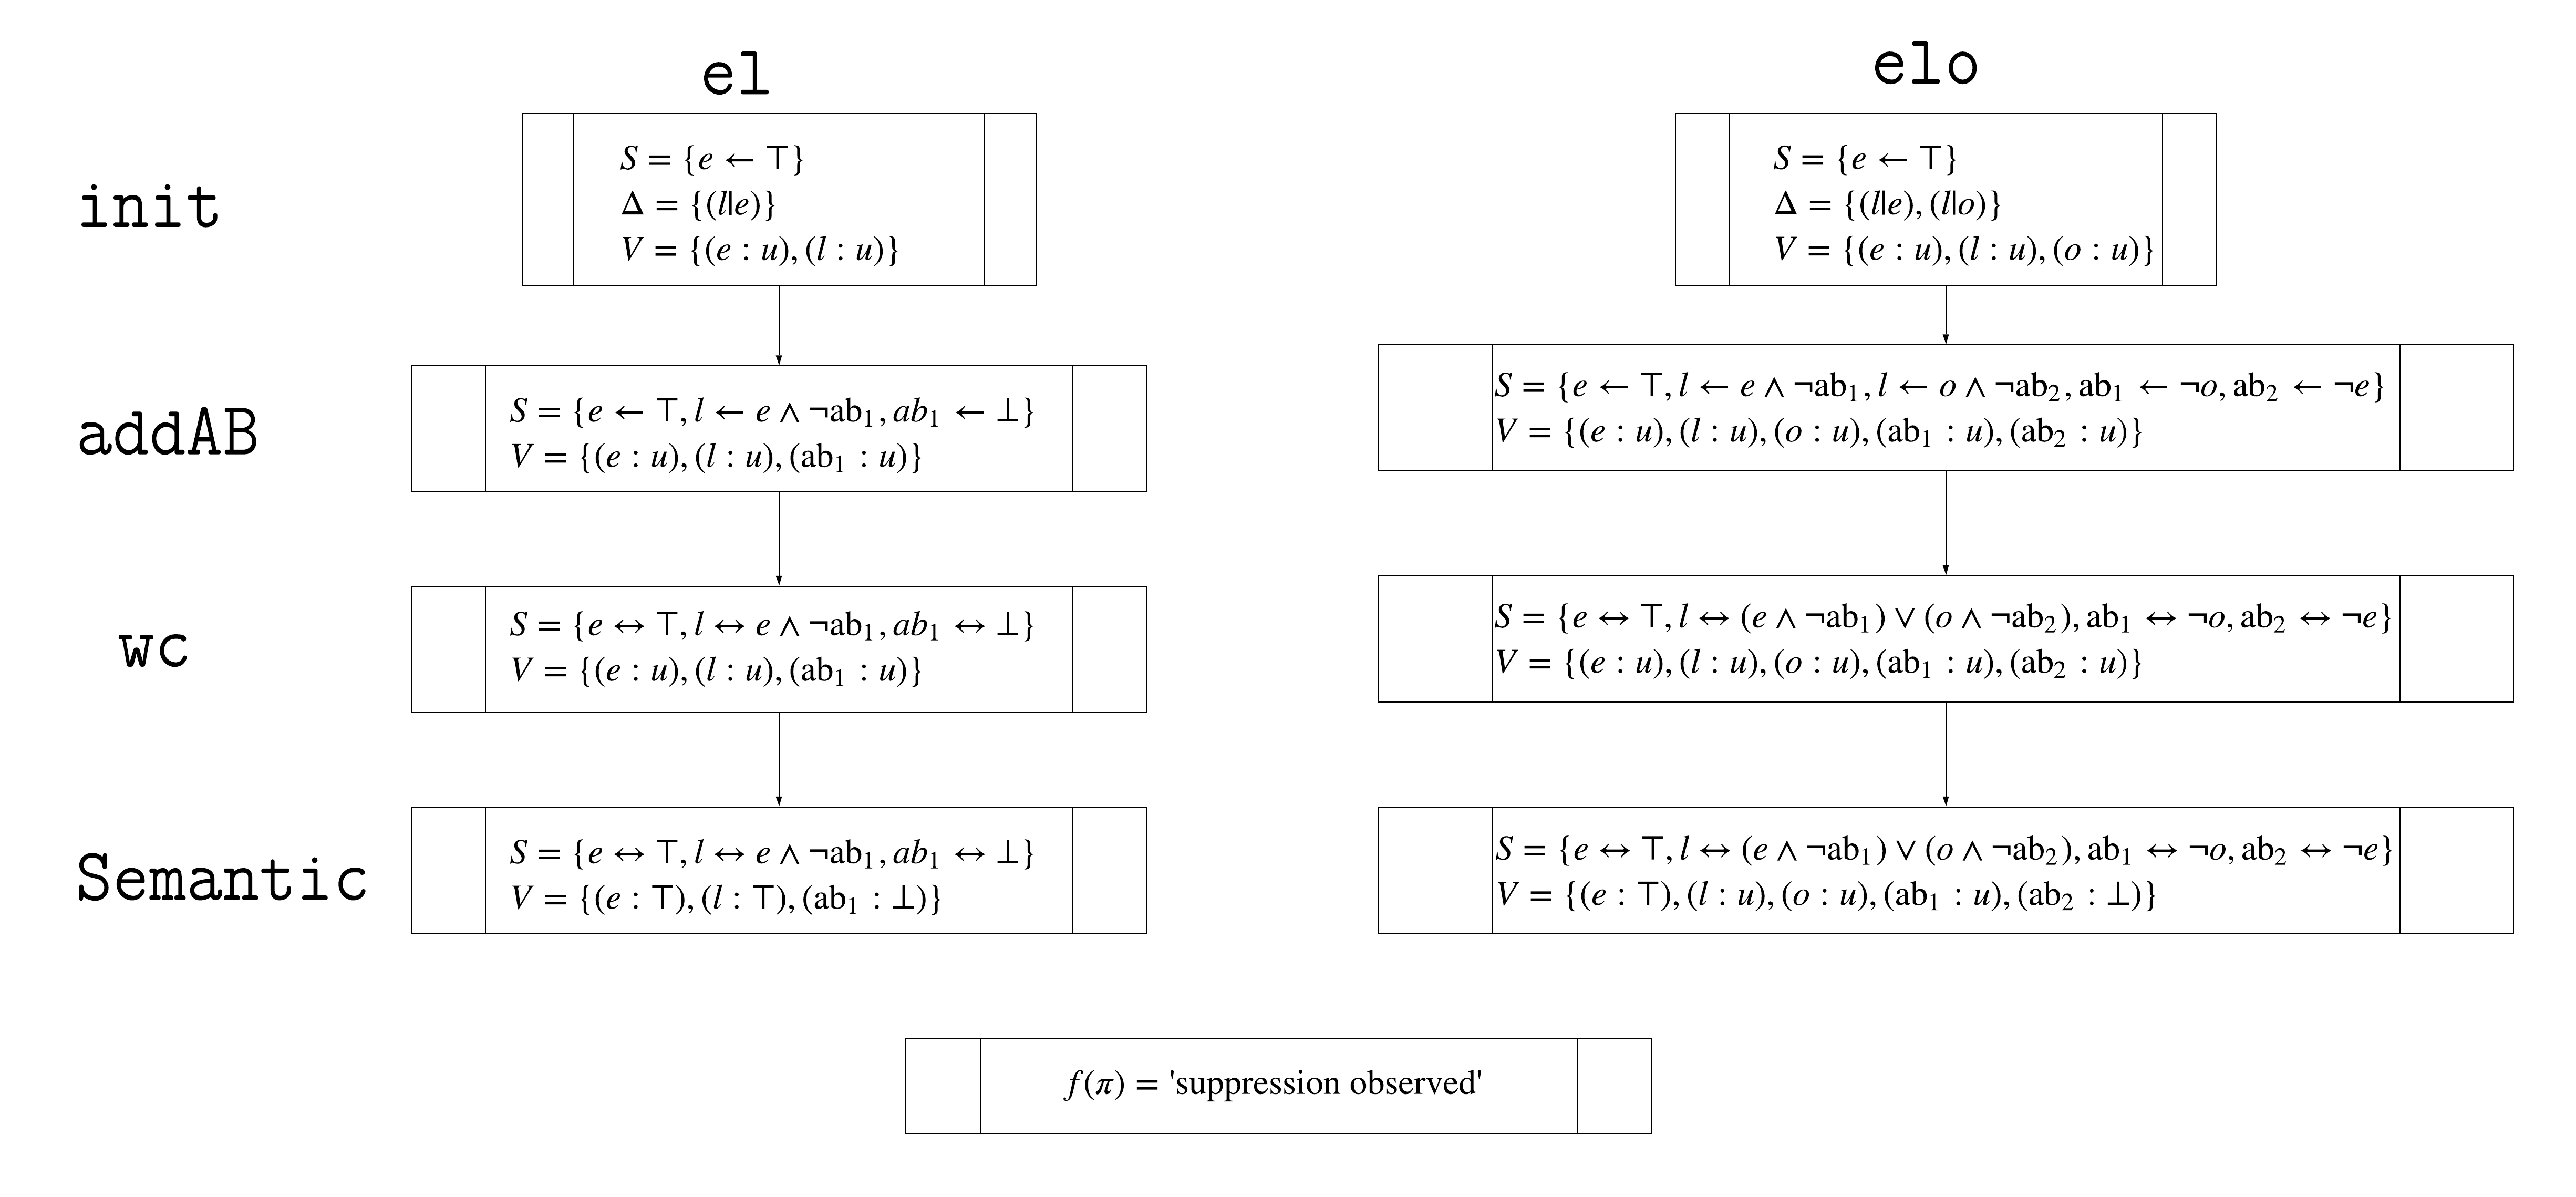
\includegraphics[width=\linewidth]{Suppression_SCP}
\caption{Suppression for the SCP $\mu_\text{sup}=(\pi=(s_i \longmapsto \texttt{addAB} \longmapsto \texttt{wc} \longmapsto \texttt{semantic}),f())$}.
\label{fig:Suppression_SCP}
\end{figure}

%==========================individual reasoners===================================

To illustrate the ability of the framework to model individual reasoners, we examine those reasoners who, despite knowing both that if she has an essay to write she will study late in the library and that if the library is open she will study late in the library, still do not demonstrate suppression, and instead draw the classical conclusion that she will study late in the library. To this end we define a second SCP Task $\Pi_\text{deviant}$.
\[\Pi_\text{deviant}=(s_\text{dev},M',f_\text{sup}(),\gamma_{\text{noSup}})\]
\[s_\text{dev}=\{s_\text{dev}^\text{el},s_\text{dev}^\text{elo}\}\]
\[s_\text{dev}^\text{el}=\{S,\Delta_\text{noSup}, V, \text{name}=\text{`el'},R\} \]
\[s_\text{dev}^\text{elo}=\{S,\Delta_\text{Sup}, V, \text{name}=\text{`elo'},R\} \]
\[
R=\{\text{delete}:\{o\}, \text{explanations}:\{o\leftarrow \top, o\leftarrow \bot\}\}
\]
Where $s_\text{dev}$ is identical to $s_i$ but includes the categorization structural variable $R$ with a sub-variables called \textit{`delete'}, and \textit{`explanations'}. 

\[M'=\{\texttt{addAB}, \texttt{semantic}, \texttt{wc}, \texttt{remove}_\bot, \texttt{addExp}\}\]

$M'$ contains $\texttt{remove}_\bot$ which is able to delete any set of variables mentioned in $R[\text{`delete'}]$ of the epistemic state. $\texttt{addExp}$ allows us to add abducible facts to an epistemic state, following the intuition we first used to model the WST in Section~\ref{ssec:wst}. To see the explanations and justifications for these two cognitive operations, refer to Section~\ref{ssec:deletion}, and Section~\ref{ssec:abd}.

Equipped with these two cognitive operations, there are several SCPs which can model $\Pi_\text{deviant}$.

Figure~\ref{fig:Suppression_SCP_del1} shows the realised SCPs for one satisfying SCP for $\Pi_\text{deviant}$. This example shows that deleting the variable $o$ from the epistemic state, prevents Suppression from occurring because the abnormality $(\text{ab}_1 \leftarrow \lnot o )$ is the cause of Suppression in $\Pi$, and in $\Pi'$ the abnormality is now given by $(\text{ab}_1 \leftarrow \lnot \top )$.

In the Appendix, Figure~\ref{fig:suppression_python} and Figure~\ref{fig:suppression_python2}  show that the non-monotonic cognitive operation \texttt{addExp} can prevent suppression by adding abducibles related to the  free variable $o$.\footnote{The output is too large to graph attractively, and should be viewed in its entirety to confirm that this approach is effective.} This is, as far as the author of this thesis is aware, the first use of \cite{holldobler2015weak}'s abducible approach to the WST to model the Suppression Task. By giving $o$ an assignment, the abnormality $(\text{ab}_1\leftrightarrow \lnot o)$ no longer evaluates to $u$, and across all final epistemic states. Together, the combined `elo' epistemic states now return every \texttt{response}() that the combined `el' epistemic states do. 

Interestingly, using $f_\text{sup()}$, the case where the abducible $(o \leftarrow \bot)$ is added, results in the previous unseen response `she will not study late in the library' to be returned in $\texttt{responses}(P_\text{elo})$ but not in $\texttt{responses}(P_\text{el})$. This is not an instance of suppression because the new response is only generated from the initial epistemic state $s_\text{dev}^\text{elo}$ whose information is a superset of the information in $s_\text{dev}^\text{el}$.

Both of these examples illustrate the derivation of the classical logical response to the suppression task as a modification of an SCP which did illustrate suppression. This evidences one of the core claims of the SCP Framework which is that it is a reasonable tool for modelling individual reasoners in a cognitive task. 

The value of these examples lies in that they show that classical logic response to a cognitive task is not necessarily derived through the use of classical logic.

\begin{figure}
\centering 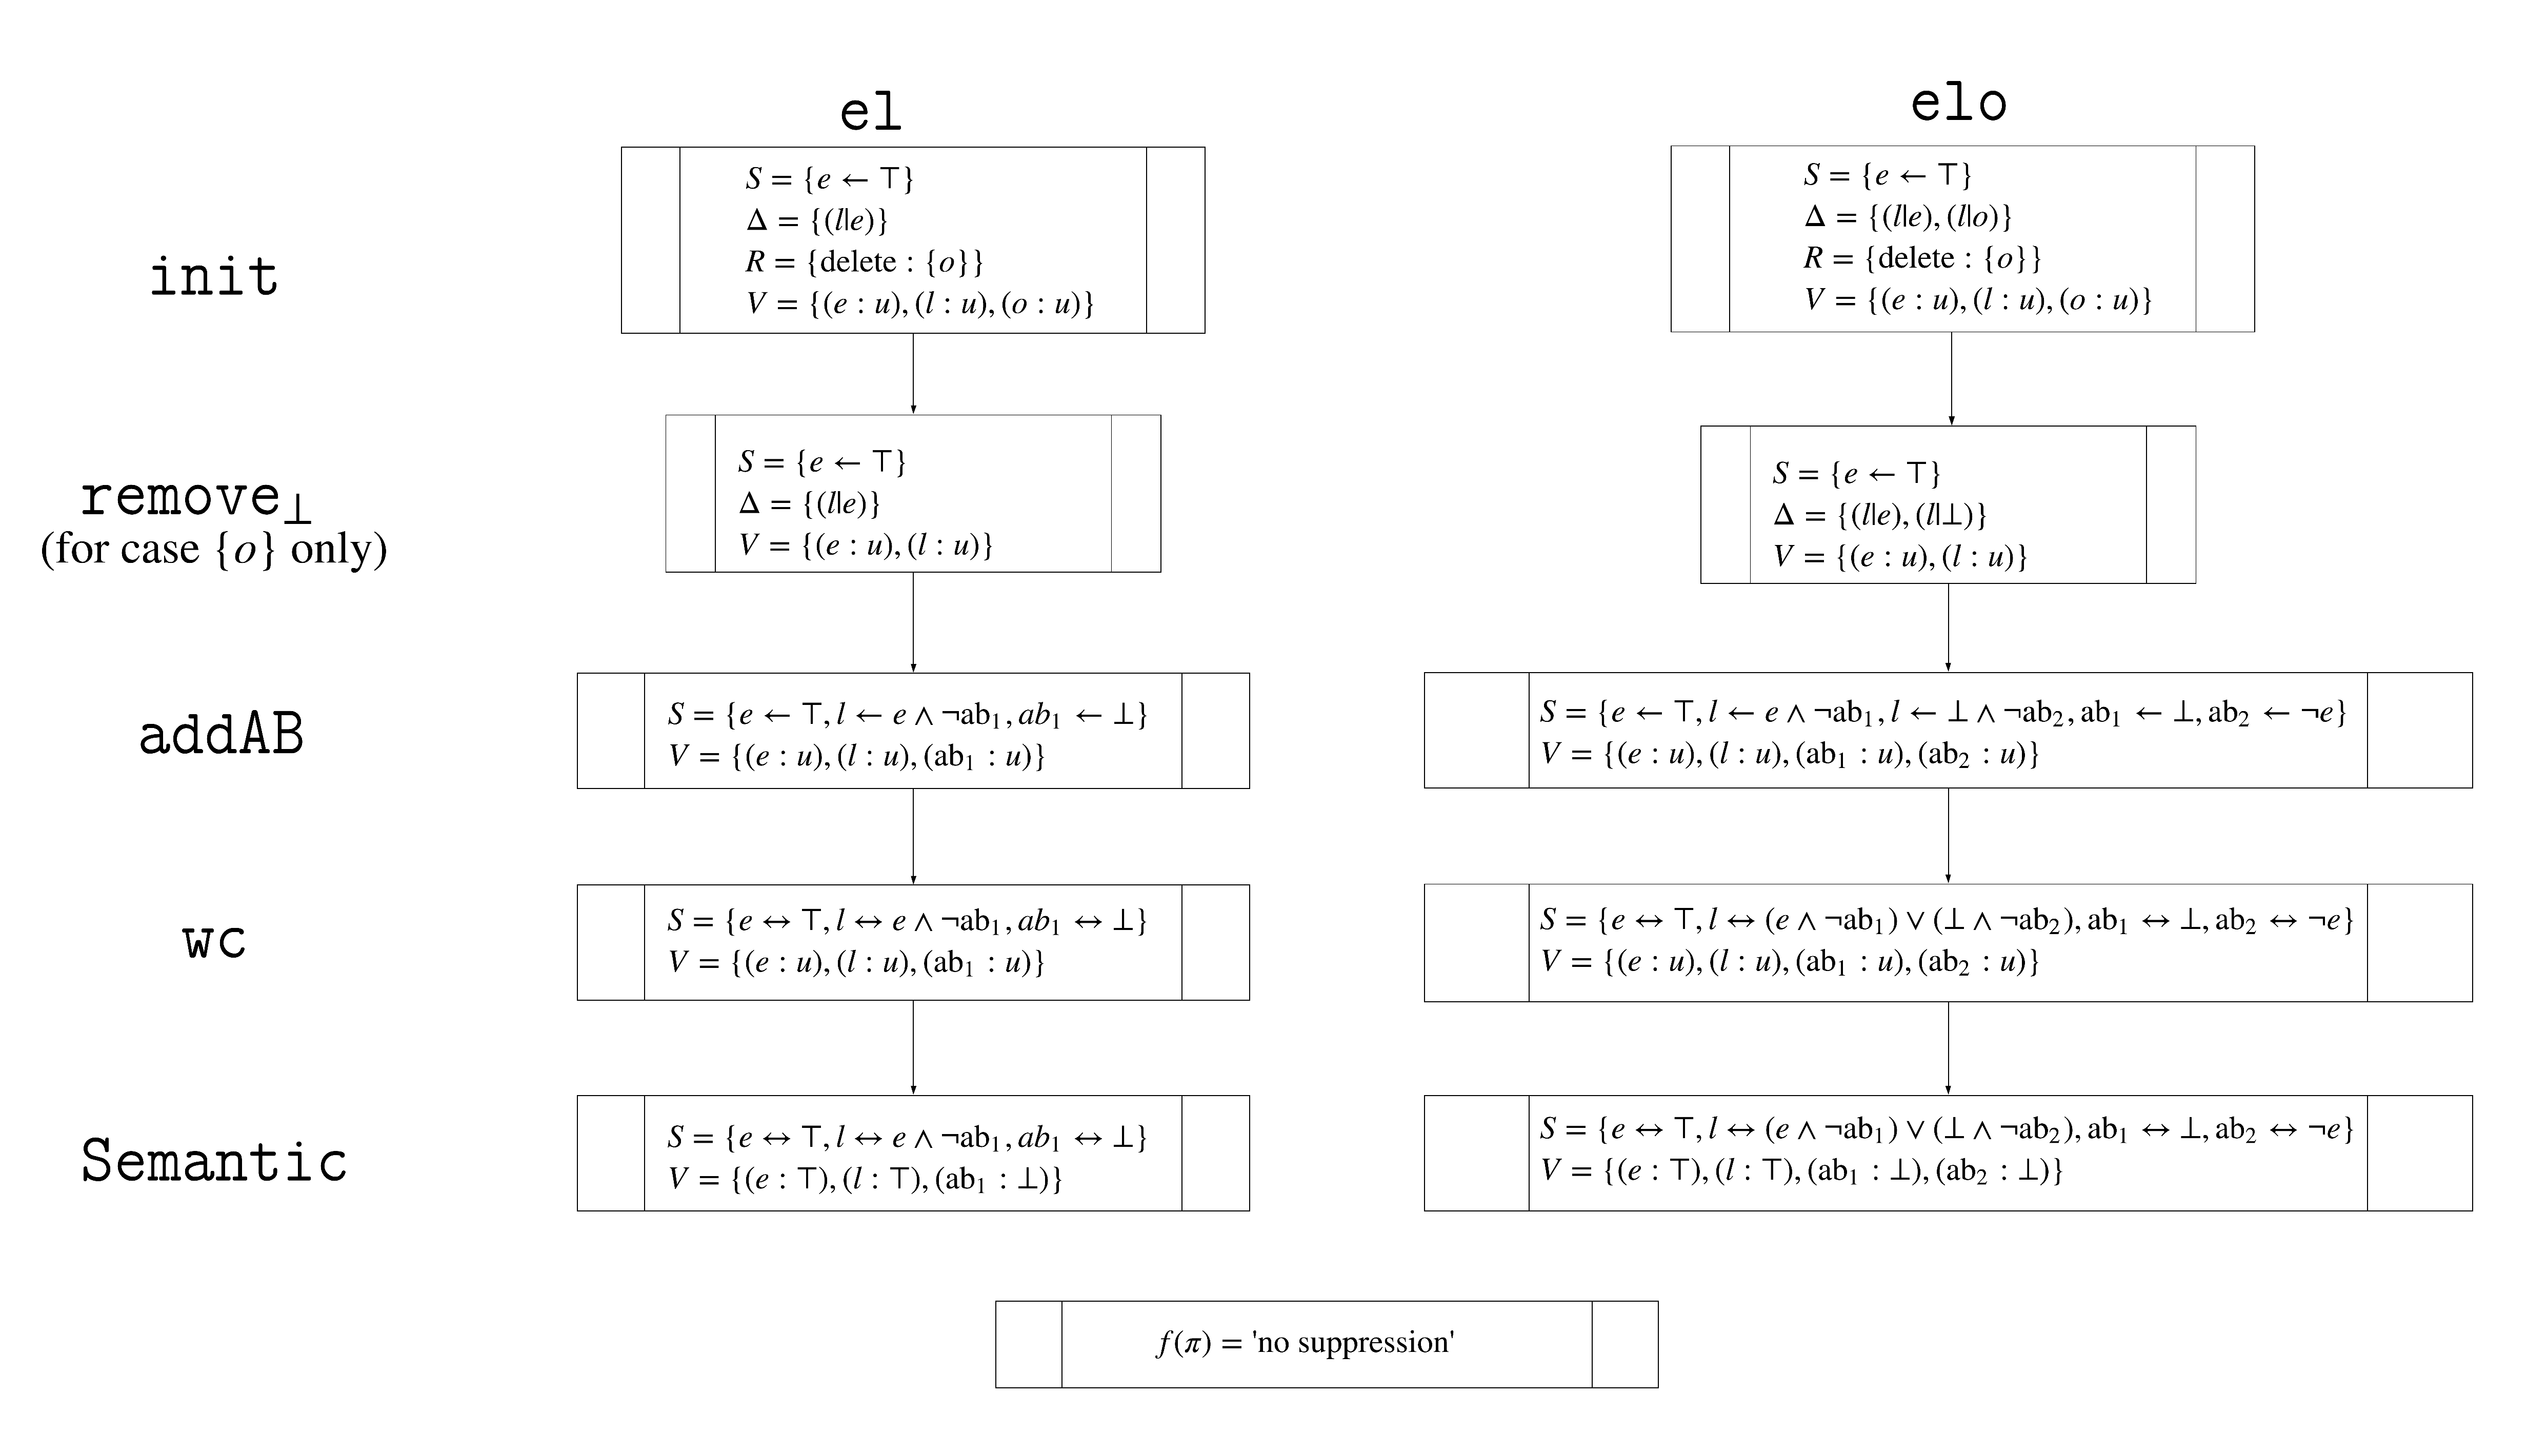
\includegraphics[width=\linewidth]{Suppression_SCP_del1}
\caption{Inhibition of Suppression for the SCP $\mu_\text{del}=(\pi,f_\text{sup}()), \pi = (s_i \longmapsto \texttt{remove}_\bot \longmapsto \texttt{addAB} \longmapsto \texttt{wc} \longmapsto \texttt{semantic}).$}.
\label{fig:Suppression_SCP_del1}
\end{figure}




\subsection{Suppression Task: Reiter's Default Logic}

As discussed in Section~\ref{ssec:supReit}, Reiter's Default Logic is not able to model the Suppression Task. This remains the case when using an SCP approximation of this logic. This brief example is provided as evidence that SCPs are able to approximate the Reiter's Default Logic interpretation of the task, rather than to propose any solutions which would make suppression possible.

In order to create this model, we introduce the new cognitive operation $\texttt{I}_W$. $\texttt{I}_W$ interprets the variable $\bar{p}[\text{`W'}]$ of input base point $\bar{p}$, and sets the variables  $\bar{p}[\text{`V'}]$ in a base point $\bar{p}'\in p'$ of the output state point $p'$ to a valid possible world configuration for those variables.


\begin{algorithm}[H]
\SetAlgoLined
\SetKwProg{Fn}{Function}{ is}{end}
\Fn{$e$($\bar{p}$)}
{
possibleAss:=$\{w|w$ is a valid possible setting of the variables in $ \bar{p}[\text{`V'}] $ for propositional knowledge base $\bar{p}[\text{`W'}]\}$\;
$p'=\{\}$\;
\For {unique $w \in $ possibleAss}
{
$\bar{p}':=\texttt{clone}(\bar{p})$\;
$\bar{p}'[\text{`V'}]:=w$\;
$p':=p' \cup \bar{p}'$\;
} 
\Return $p'$
}
\caption{$\texttt{I}_w$ generates possible world assignments for a propositional knowledge base $W$.}
 \label{alg:I}
\end{algorithm}

Equipped with this new cognitive operation we might define the SCP Task $\Pi_\text{default}$ as follows:
\[\Pi_\text{default}=(s_d,M_d,f_\text{sup}(),\gamma_\text{sup})\]
\[s_d=\{s_d^{el}, s_d^{elo}\}\]
\[s_d^{el}=(W,D_{el},V_{el})\]
\[s_d^{elo}=(W,D_{elo},V_{elo})\]
Where the initial state $s_d$ consists of epistemic states containing the initial information that she will study late in the library, as well as extra conditional information interpreted as a set of defaults, as in Section~\ref{ssec:supReit}, and a possible world variable. Each epistemic state in the initial state point encodes the information required to form a default theory of the form $(W,D)$.
\[W=\{e\leftarrow \top\}\]
\[
D_{el}=\{\delta_1:\frac{e\leftarrow \top:\text{ab}_1 \leftarrow \bot}{l\leftarrow\top} ,
\delta_2:\frac{\top:\text{ab}_1 \leftarrow \top}{\text{ab}_1\leftarrow\top}
\}
\]
\[
D_{elo}=\{\begin{matrix}\delta_1:\frac{e\leftarrow \top:\text{ab}_1 \leftarrow \bot}{l\leftarrow\top} ,
\delta_2:\frac{o\leftarrow \top:\text{ab}_2 \leftarrow \bot}{l\leftarrow\top},
\delta_3:\frac{o\leftarrow \bot:\text{ab}_1 \leftarrow \top}{\text{ab}_1\leftarrow\top},
\delta_4:\frac{e\leftarrow \bot:\text{ab}_2 \leftarrow \top}{\text{ab}_2\leftarrow\top}
\end{matrix}\}
\]
\[V_{el}=\{(e,u),(l,u)\}\]
\[V_{elo}=\{(e,u),(l,u), (o,u)\}\]
To show the use of SCPs in the default logic interpretation of the suppression task, we limit the set of allowable cognitive operations $M_d$ as follows:
\[M_d=\{\texttt{default},\texttt{I}_w\}\]
De Novo search reveals no satisfying SCPs for $\Pi_\text{default}$, as we would expect from a faithful adaptation of Reiter's Default Logic which is unable to demonstrate suppression. The modified SCP Task $\Pi'_\text{default}=(s_d,M_d,f_\text{sup}(),\gamma_\text{noSup})$, does have a satisfying SCP.

\[\mu'_d=(\pi'_d, f_\text{noSup})\]
\[\pi'_d=(s_d \longmapsto \texttt{default} \longmapsto \texttt{I}_W)\]
We find that suppression is not observed. We define the final state points of the epistemic states $s_d^{el}$ and $s_d^{elo}$ which we will call $P^{el}$ and $P^{elo}$, respectively. We find that $(l, \top) \in P^{el}_i$, and $(l, \top) \in P^{elo}_j$ for every base point $P^{el}_i \in_S P^{el}$ and $P^{elo}_i \in_S P^{elo}$. For this reason, $f_\text{sup}(\pi'_d) \models \gamma$. 

These results mimic the intuition and data transformations steps used in Section~\ref{ssec:supReit}, but do so in a more structured way. When considered in conjunction with the SCP generated for the WST interpretation of the Suppression Task, the simplicity of the SCP framework for modelling cognitive tasks across different logics is evident.

\section{Wason Selection Task}\label{sec:wstSCP}



In order to model the abstract case of the WST, we define the SCP Task $\Pi=(s_i,M,f_\text{WST}(),\gamma)$. $\Pi$ is intended to model the most most common card choice made by reasoners: turning both $D$ and $3$. The choice of external evaluation function for this task (the turn function), if we are to follow the intuition from Section~\ref{ssec:sup_mod}, has two requirements: it must be able to capture whether an observation $O$ can be explained by the least model of the weakly completed program, and it must ensure that variable assignments which could falsify or verify the conditional rule $(3|D)$ using our \textit{de Finetti} truth table (Table~\ref{tbl:cond}), are present in the least model. 

To this end, we add a set of abducibles to the categorization variable $R$, and combine this with the variables for the set of propositional rules $S$, conditional rules $\Delta$, and possible world $V$ to create the initial state point $s_i$.

Next, we require an intuition for the contents of $s_i$. In this case, abduction can be simulated by the SCP in one of three ways. The first is to create a unique SCP for each possible explanation for each observation as we did for the classical WCS interpretation of the task in Section~\ref{ssec:sup_mod}. But the fact that SCPs may contain an initial state point, rather than just a single epistemic state, enables a more elegant solution that captures the full scope of possible (\textit{observation}, \textit{explanation}) pairings. The other two options are to start with a state point containing each abductive case, or to create cognitive operations which add the abducible cases at computation time. Opting for the latter, we define:

\[
s_i=(S,\Delta, R)
\]
\[
S=\{\}
\]
\[
\Delta=\{(3|D)\}
\]
\[
R=\{\text{abducibles}:\{D\leftarrow \top, D \leftarrow \bot, K\leftarrow \top, K \leftarrow \bot, 3\leftarrow \top, 3 \leftarrow \bot, 7\leftarrow \top, 7\leftarrow \bot\}\}
\]

Because SCPs aim to capture as much cognitive information as possible within the CTM as possible, we will prefer this third case and make use of the categorization variable $R$ to specify both the set of abducibles, and, later, the chosen explanations $(\epsilon)$. In Section~\ref{cogOp:addExp} we defined the complex operation $\texttt{addExp}$ which creates a new epistemic state as output for each possible combination of the abducibles that could be added to $\bar{p}[\text{'S'}]$ of input base point $\bar{p}$.

For the purposes of readability, we will restrict examination of the abducibles to cases that are of length 1, and contain only positive facts\footnote{A reader wishing to see this process with respect to the full set of abducibles should examine the \texttt{WST.py} file in the SCP implementation.}.

Next, we define the final state dependent external evaluation function $f_\text{WST}()$ as follows:

\begin{algorithm}[H]
\SetAlgoLined
\SetKwProg{Fn}{Function}{ is}{end}
\Fn{$\texttt{f}_\text{WST}(\pi)$}
{
\tcc{This is a final state evaluation SCP.}
Let $R=[(k \in K[\pi],f())]$ be the set of realised SCPs $r_i=(k,f())$ which can be generated from $\pi$\;
Let $P=[\bar{p}_1,...,\bar{p}_n]$, where $\bar{p}_i$ is the final epistemic state of $r_i$\;
Let $\epsilon=[\epsilon_1,...,\epsilon_n]$, where $\epsilon_i=\bar{p}_i[R][\text{`}\epsilon\text{'}]$\;
Let $O=\{(D,\top),(K,\top),(3,\top),(7,\top)\}$ be the set of observations\;
\tcc{We include the contrapositive case $(D' | 7)$ because it will be shown to be useful in modelling individual reasoners later.}
Let $C=\{(3|D), (D' | 7)\}$ be the set of conditionals which must be falsified or verified\;
Output=\{\}\;
\For{$\bar{p}_i \in P$}
{
run \texttt{isExplanation}($\bar{p}_i,O$)\;
}

\For{each minimal explanation $e$ for observation $o$}
{
\uIf {$I_\text{e[{`V'}]}(C)$ either falsifies or verifies some conditional in $C$}
{
Output[o]:=Output[o]$\cup$ `Turn Card'\;
}
\Else
{
Output[o]:=Output[o]$\cup$ `Do not turn Card'\;
}
}

\Return Output
}
\Fn{$\texttt{isExplanation}(\bar{p}_i,O)$}
{
\For {each $o \in O$}
{
\If{$I_{\bar{p}_i[\text{`V'}]}(\bar{p}_i[\text{`S'}]) \models o$}
{
\tcc{Then $\bar{p}_i$ explains $o$.}
Add $\bar{p}_i$ to the explanations for $o$.
}
}
}

\caption{$\texttt{f}_\text{WST}$}
 \label{f:wst}
\end{algorithm}

\begin{sidewaysfigure}
\centering{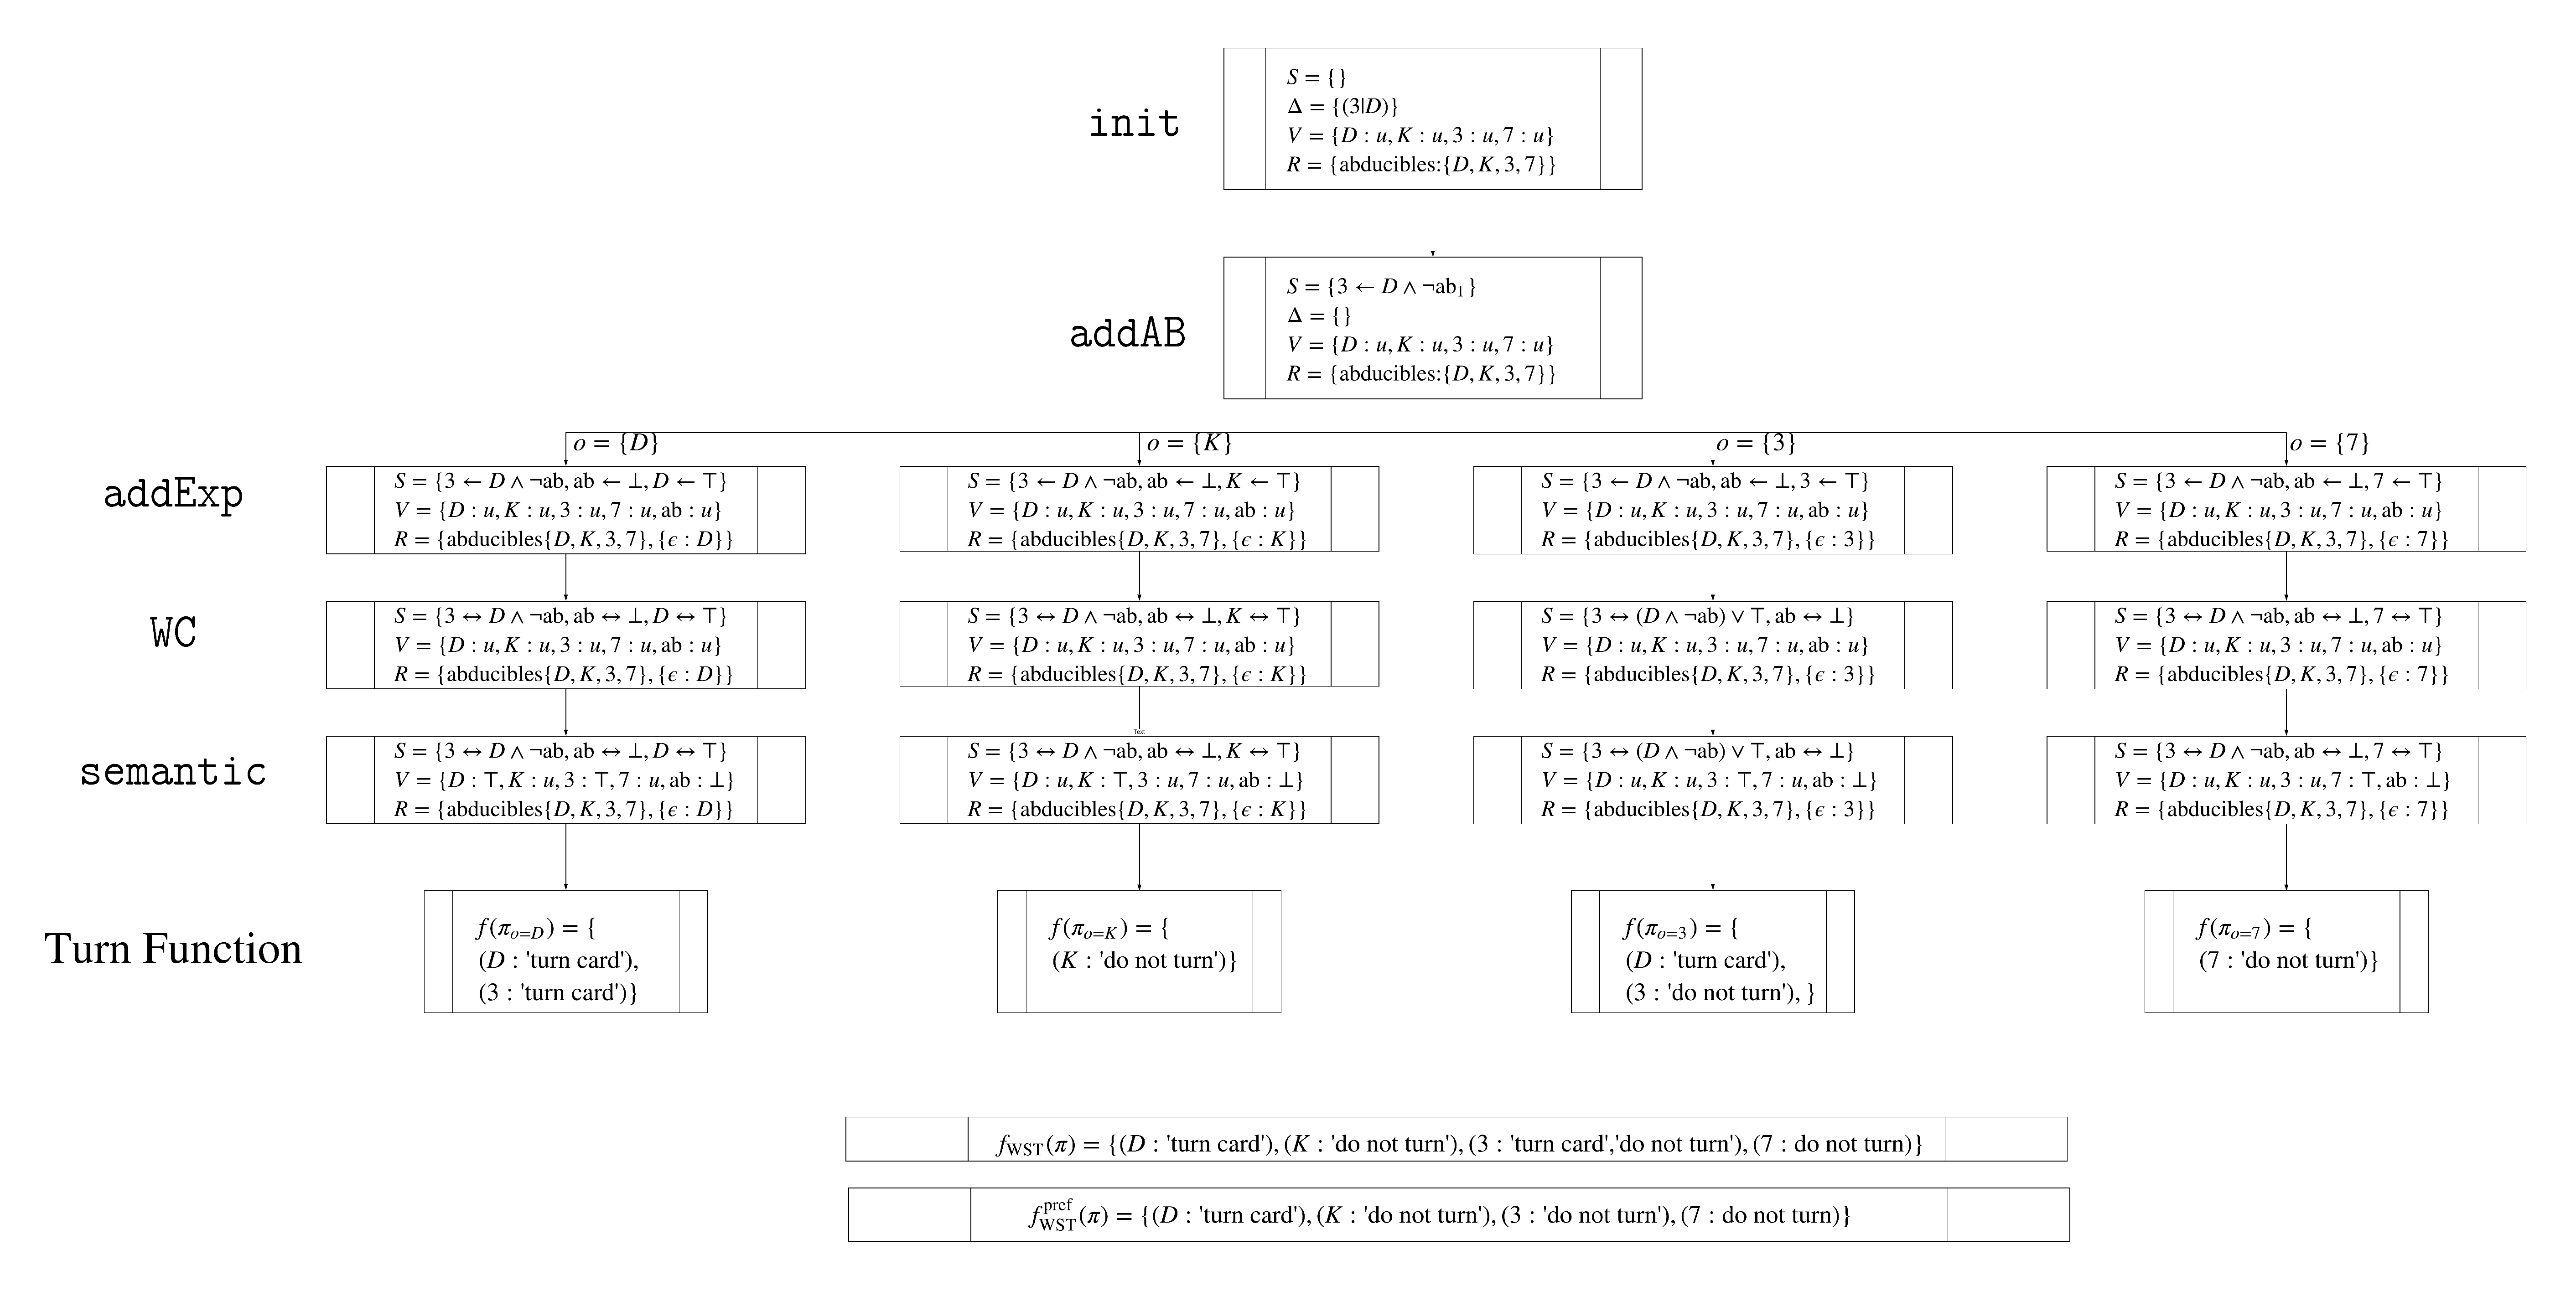
\includegraphics[width=\linewidth]{realisedSCPsWST}}

\caption{Realised SCPs for the SCP interpretation of the WST where $\mu_{D,3}=(\pi,f_\text{WST})$, and $\mu_D=(\pi,f_\text{WST}^\text{pref})$, with $\pi=(s_i \longmapsto \texttt{addAB} \longmapsto \texttt{addExp}  \longmapsto \texttt{wc} \longmapsto \texttt{semantic})$. Results for $\mu_\{D,3\}$ mimic those observed in \cite{holldobler2015weak}'s WST interpretation which concludes the canonical case $D,3$. Results for $\mu_{D}$ conclude the canonical case $D$. }
\label{fig:rSCP_WST}
\end{sidewaysfigure}

Next we create our goals. We will make one goal for each of the canonical cases of the WST. The structure of the goal associates a turn function with every possible observation that needs to be explained.
\[\gamma_{D,3}=\{(\text{D}:\text{turn card}),(\text{3}:\text{turn card}),(\text{K}:\text{do not turn}),(\text{7}:\text{do not turn})\}\]
\[\gamma_{D}=\{(\text{D}:\text{turn card}),(\text{3}:\text{do not turn}),(\text{K}:\text{do not turn}),(\text{7}:\text{do not turn})\}\]
\[\gamma_{D,7}=\{(\text{D}:\text{turn card}),(\text{3}:\text{do not turn}),(\text{K}:\text{do not turn}),(\text{7}:\text{turn card})\}\]
\[\gamma_{D,3,7}=\{(\text{D}:\text{turn card}),(\text{3}:\text{turn card}),(\text{K}:\text{do not turn}),(\text{7}:\text{turn card})\}\]
Next, we define the set of allowable cognitive operations $M$. In this case, because our previous modelling of the general case of the WCS required the addition of explanations from the set of abducibles, we will include the operation \texttt{addExp} (as seen in the SCP Modelling of individual cases of the Suppression Task).
\[M=\{\texttt{addAB}, \texttt{semantic}, \texttt{wc}, \texttt{AddExp}\}\]
The overall planning task, $\Pi$, can now be formulated for the general case of the WST.
\[\Pi=(s_i,M,f_\text{WST}(),\gamma_{D,3})\]
De Novo search for the SCP Plan yields several SCP (differentiated by where the \texttt{addExp} cognitive operation occurs), including this one:
\[\mu_{D,3}=(\pi,f_\text{WST}())\}\]
\[
\pi=(s_i\longmapsto \texttt{addAB} \longmapsto \texttt{addExp} \longmapsto \texttt{wc} \longmapsto \texttt{semantic})
\]
\[
f_\text{WST}(\pi)=
\left\lbrace
\begin{matrix}
(\text{D}:\{\text{turn card},\text{do not turn}\}), & 
(\text{3}:\{\text{turn card},\text{do not turn}\}), \\
(\text{K}:\{\text{do not turn}\}), &
(\text{7}:\{\text{do not turn}\})
\end{matrix}
\right\rbrace
\]



Figure~\ref{fig:rSCP_WST} demonstrates the calculation of $f(\pi)$ for each positive explanation $\epsilon$ of length 1. When this task is run for minimal explanations of unrestricted length, the set of conclusions for each card returned by $f_\text{WST}()$ do not change. We find that $\mu_{D,3}\models_\text{weak} \gamma_{D,3}$ and that we should turn the cards $D$, and $3$, precisely as in \cite{dietz2014modeling}'s model. In the figure the partial turn function $f_{\pi_{o=x}}$ means: `if $x$ were the only observation in O, what would be the result of $f_\text{WST}(\pi)$?'. It is provided only for illustrative purposes.

Thus, it has been shown that the SCP Framework is capable of modelling the general response to the abstract case of the WST.

%---------------------------------------Extensions---------------------------------------

In order to model the goals $\gamma_{D}$, $\gamma_{D,7}$, and $\gamma_{D,3,7}$, we must again change our SCP Task. These extensions are easily introduced and, the author hopes, will serve as motivation of the practical and intuitive usefulness of the SCP Framework.

The simplest of these case to model is  $\gamma_{D}$. This could done by creating the new SCP Task $\Pi_D$.

\[
\Pi_D = (s_i, M, \gamma_D, f_\text{WST, simple})
\]

And defining $f_\text{WST, simple}$ precisely as $f_\text{WST}$ was defined, except that the \texttt{isExplanation} function in Algorithm~\ref{alg:outPutcondition} is changed to that of 
Algorithm~\ref{alg:outPutconditionModified}.

\begin{algorithm}[H] 
\SetAlgoLined
\SetKwProg{Fn}{Function}{ is}{end}
\Fn{$\texttt{isExplanation}(\bar{p}_i,O)$}
{
\For {each $o \in O$}
{
\If{$I_{\bar{p}_i[\text{`V'}]}(\bar{p}_i[\text{`S'}]) \models o$}
{
\tcc{Then $\bar{p}_i$ explains $o$.}
Add $\bar{p}_i$ to the explanations for $o$.
}
}
}
\caption{\texttt{isExplanation} function as it appears in $\texttt{f}_\text{WST}$.}
\label{alg:outPutcondition}
\end{algorithm}

\begin{algorithm}[H] 
\SetAlgoLined
\SetKwProg{Fn}{Function}{ is}{end}
\Fn{$\texttt{isExplanation}(\bar{p}_i,O)$}
{
\For {each $o \in O$}
{
\tcc:{We require that the observation being explained is an element of the proposed explanations.}
\If{$I_{\bar{p}_i[\text{`V'}]}(\bar{p}_i[\text{`S'}]) \models o$ AND $o \in \bar{p}_i[\text{`R'}][\text{`}\epsilon\text{'}]$}
{
\tcc{Then $\bar{p}_i$ explains $o$.}
Add $\bar{p}_i$ to the explanations for $o$.
}
}
}
\caption{\texttt{isExplanation} function as it appears in $\texttt{f}_\text{WST, simple}$.}
\label{alg:outPutconditionModified}
\end{algorithm}

This approach mimics the logic we used to create the Simple WCS Extension in Section~\ref{sec:sup}. However, there is an alternative approach which the author prefers. 

One should note that, while $\mu_{D,3}\models_\text{weak} \gamma_{D,3}$, it is also the case that that `do not turn' occurs in $f_\text{WST}(\pi)[K]$, $f_\text{WST}(\pi)[3]$, and $ f_\text{WST}(\pi)[7]$, but is not in $ f_\text{WST}(\pi)[D]$. If we treat $f_\text{WST}(\pi)$ sceptically and assume that we only turn a card if there is \textit{no reason not to turn it}, we arrive at the conclusion that only $D$ should be turned.

We define a set of preferred responses which prefers the `do not turn' response as follows (using preferred responses as defined in Section~\ref{ssec:f}):
\[
\text{pref}=\{(\text{D}:\text{do not turn}),(\text{3}:\text{do not turn}),(\text{K}:\text{do not turn}),(\text{7}:\text{do not turn})\}
\]
\[
p(f_\text{WST}(\pi),\text{pref})=\{(\text{D}:\text{turn card}),(\text{3}:\text{do not turn}),(\text{K}:\text{do not turn}),(\text{7}:\text{do not turn})\}
\]
Now it is clear that $p(f_\text{WST}(\pi),\text{pref})= \gamma_D$. To return this to an acceptable SCP format, we may simply define $f_\text{WST}^\text{pref}=p(f_\text{WST}(\pi)$ and observe that $\mu_D \models \gamma_D$ for SCP $\mu_D=(\pi, f_\text{WST}^\text{pref}())$. Figure~\ref{fig:rSCP_WST} illustrates the process by which the canonical case $D$ is derived.
%------------------Contraposition-----------------------------------


\begin{sidewaysfigure}
\centering{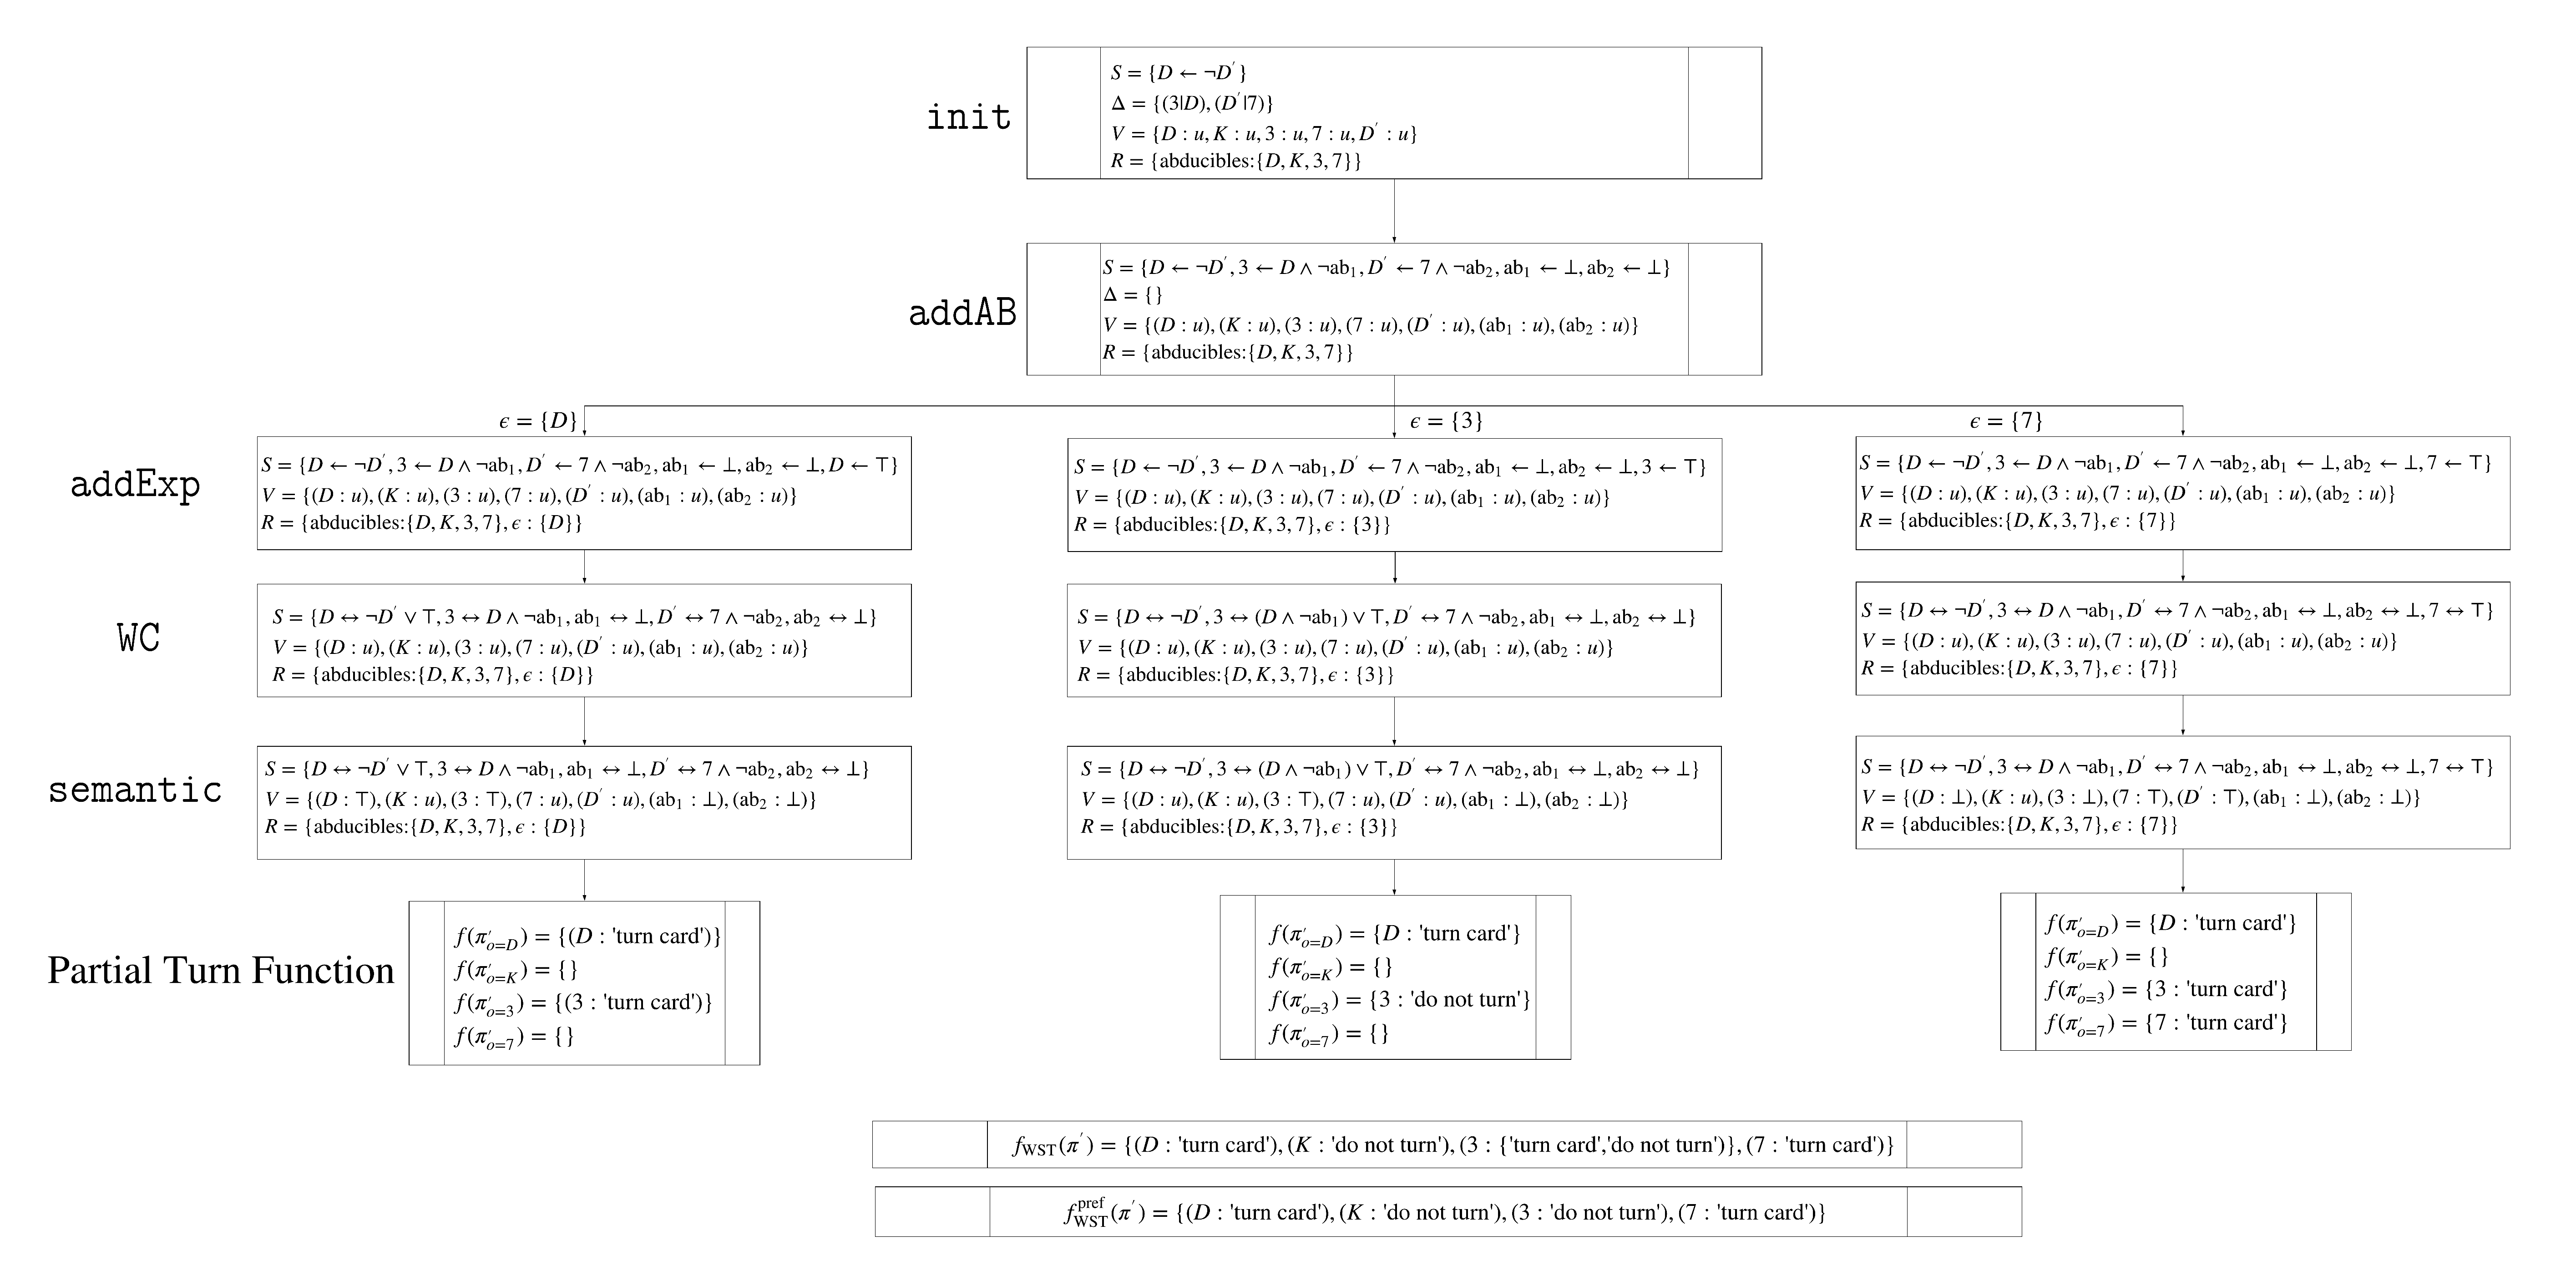
\includegraphics[width=\linewidth]{realisedSCPsWST_mod}}

\caption{Realised SCPs for the SCP interpretation of the WST where $\mu_{D,3,7}=(\pi',f_\text{WST})$, and $\mu_{D,7}=(\pi',f_\text{WST}^\text{pref})$, with $\pi=(s_i' \longmapsto \texttt{addAB} \longmapsto \texttt{addExp}  \longmapsto \texttt{wc} \longmapsto \texttt{semantic})$.  Results for $\mu_{D,3,7}$, $\mu_{D,7}$ conclude the canonical cases $\{D,3,7\}$ and $\{D,7\}$, respectively. The case for $\epsilon=\{K\}$ is omitted, for reasons of readability.}
\label{fig:realisedSCPsWST_mod}
\end{sidewaysfigure}


Implementing contraposition in the SCP framework we have defined is surprisingly simple. We simply need to define a new SCP Task $\Pi_\text{D,3,7}$ as follows:
\[
\Pi_\text{D,3,7} = (s_i', M, \gamma_{D,3,7}, f_\text{WST}())
\]
\[
s_i'=(S', \Delta', R)
\]
\[
S'=\{(D \leftarrow \lnot D')\}
\]
\[
\Delta'=\{(3|D),(D'|7)\}
\]

Simply by adding the contrapositive conditional and its variable initialization, search returns an SCP $\mu_{D,3,7}=(\pi', f_\text{WST}())$, $\pi'=(s_i' \longmapsto \texttt{addAB} \longmapsto \texttt{addExp} \longmapsto \texttt{wc} \longmapsto \texttt{semantic})$, with $f_\text{WST}(\pi')\models_\text{weak} \gamma_{D,3,7}$. It is worth noting that $\pi$ and $\pi'$ differ only in the contents of their respective initial state points.

%Figure~@TODO illustrates this fact for positive explanations of length 1.

Finally, the case where the $D$ and $7$ cards are turned (the classical inference), can be modelled by combining aspects of the SCPs above. We define the SCP Task $\Pi_\text{D,7}$:


\[
\Pi_\text{D,7} = (s_i', M, f_\text{WST}^\text{pref}(), \gamma_{D,7})
\]

And running De Novo search over this Task reveals that the SCP $\mu_{D,7}=(\pi', f_\text{WST}^\text{pref}())$ is a satisfying SCP for the goal $\gamma_{D,7}$. %Figure~@TODO illustrates this point.



Figure~\ref{fig:realisedSCPsWST_mod} illustrates $\mu_{D,3,7}$ and $\mu_{D,7}$, and demonstrates that only the external evaluation function differs between them. The interested reader is also pointed to \texttt{example\_wcs\_wst.py}, where they can see this process for the full set of abducibles and should note some of the interesting effects of negative explanations on the turn functions.

Thus, it has been shown that two CTMs $\pi$, and $\pi'$, in conjunction with the external activation functions $f_\text{WST}()$ and $f_\text{WST}^\text{pref}()$ are able to model individual reasoners in the Wason Selection Task for all four of the canonical cases.













